\sectioncounter{11}
  \section{导数的定义和计算}

  \subsection{知识梳理}
  对瞬时速率和切线斜率的研究产生了导数的概念. 设路程 $s$ 是关于时刻 $t$ 的函数, 记为 $s(t)$, 则在时间段 $[t,t_1]$ 内的平均速率为 
  $\frac{s(t_1)-s(t)}{t_1-t}$. 令 $t_1\to t$, 这个平均速率就化为在 $t$ 时刻的瞬时速率. 
  
  求函数 $y=f(x)$ 的图象在点 $P(x_0,f(x_0))$ 处切线的斜率也可用相同的方法. 先在点 $P$ 附近取另一点 $Q(x_1,f(x_1))$, 求割线 $PQ$ 的斜率 
  $\frac{f(x_1)-f(x)}{x_1-x}$. 令 $x_1\to x$, 割线 $PQ$ 的斜率就化为点 $P$ 处切线的斜率 (如图 \ref{fig-191127-2145}). 
  \begin{figure}[htb]
    \small
    \centering
    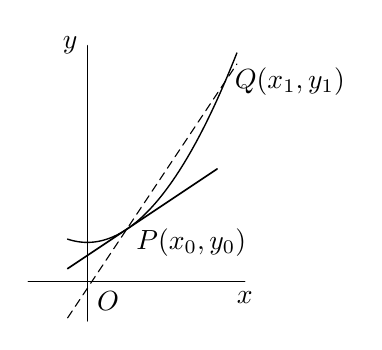
\begin{tikzpicture}[line cap=round,line join=round,scale=0.5]
      \draw[\myaxisarrow] (-1.5,0) -- (4,0) node[below] {$x$};
      \draw[\myaxisarrow] (0,-1) -- (0,6) node[left] {$y$};
      \draw[line width=0.5pt,smooth,samples=100] 
        plot[domain=-0.5:3.8](\x,{(\x)^2/3+1});
      \draw[line width=0.6pt,smooth,samples=100] 
        plot[domain=-0.5:3.3](\x,{(2*\x+2)/3});
      \draw[line width=0.4pt,smooth,samples=100,densely dashed] 
        plot[domain=-0.5:3.8](\x,{3*\x/2-1/6});
      \draw (0,0) node[anchor=north west] {$O$}
        (1,1) node[right] {$P(x_0,y_0)$}
        (3.5,{61/(12)}) node[right] {$Q(x_1,y_1)$};
    \end{tikzpicture}
    \caption{}\label{fig-191127-2145}
  \end{figure}

  函数 $f(x)$ 的\myindex{导函数} (derivative, 简称导数) $f'(x)$ 定义为
  \[f'(x)=\lim_{x_1\to x} \frac{f(x_1)-f(x)}{x_1-x}
    = \lim_{\Delta x\to 0} \frac{f(x+\Delta x)-f(x)}{\Delta x}.\]
  计算基本初等函数的导数时, 常用后一式. 例如求函数 $f(x)=x^2$ 和 $g(x)= \frac1x$ 的导数时,
  \[\frac{f(x+\Delta x)-f(x)}{\Delta x}= 2x+\Delta x,\quad
    \frac{g(x+\Delta x)-g(x)}{\Delta x}= -\frac1{x(x+\Delta x)},\]
  则 $f'(x)=2x$, $g'(x)= -\frac1{x^2}$, 即
    \[(x^2)'=2x,\quad (x^{-1})'=-x^{-2}.\]

  常见函数的导数公式如下:
  \mymarginpar{ $\sin x$ 与 $\cos x$ 导数公式也可写为
  \begin{gather*}
    (\sin x)'= \sin\Big(x+\frac{\pi}2\Big),\\
    (\cos x)'= \cos\Big(x+\frac{\pi}2\Big).
  \end{gather*}}
  \begin{gather*}
    (x^\alpha)'= \alpha x^{\alpha-1},\quad
    (\mathrm{e}^x)'= \mathrm{e}^x,\quad
    (\ln x)'= \frac1x,                               \\
    (\sin x)'= \cos x,\quad  (\cos x)'= -\sin x.
  \end{gather*}
  导数还有如下计算法则:
  \mymarginpar{三个函数 $f$, $g$, $h$ 乘积的导数
  \[(fgh)'= f'gh+fg'h+fgh'.\]
  上式可推广到 $n$ 个函数乘积的导数, 由此知 $(x^n)'=nx^{n-1}$.}
  \begin{gather*}
    (Cf)'= Cf',\quad  (f\pm g)'= f'\pm g',\\
    (fg)'= f'g+fg',\quad  \Big(\frac{f}g\Big)'= \frac{f'g-fg'}{g^2},
  \end{gather*}
  其中 $f$, $g$ 为函数, $C$ 为常数. 注意, $\Big(\frac{x}2\Big)'= \frac12(x)'= \frac12$, 可简化运算.

  \lianxi
  \begin{exercise}
    若 $f(x)=x^4$, $g(x)=\frac1{\sqrt{x}}$, 求 $f'(x)$, $g'(x)$.
  \end{exercise}

  \beginsolution
    $f'(x)=4x^3$, 由 $g(x)=x^{-\frac12}$ 知 $g'(x)=-\frac12 x^{-\frac32}$.
  \endsolution
  
  \begin{exercise}
    求函数 $y=x+ \frac1x$ 的导数.
  \end{exercise}

  \beginsolution
    由 $y=x+x^{-1}$ 知 $y'=1-x^{-2}$.
  \endsolution
  
  \begin{exercise}
    求函数 $y=3\sin x\cos x+4$ 的导数.
  \end{exercise}

  \beginsolution
    $y'=3\cos x\cos x+3\sin x(-\sin x)= 3(\cos^2 x-\sin^2 x)$.
  \endsolution
  
  \begin{exercise}
    求函数 $f(x)= \frac{\mathrm{e}^x}x$ 的导数.
  \end{exercise}

  \beginsolution
    方法一: $f'(x)=\frac{\mathrm{e}^x\cdot x-\mathrm{e}^x}{x^2}
      = \frac{\mathrm{e}^x(x-1)}{x^2}$.
      
    方法二: 由 $f(x)=\mathrm{e}^x x^{-1}$ 知
    \[f'(x)=\mathrm{e}^x x^{-1}+\mathrm{e}^x (-x^{-2})
      = \frac{\mathrm{e}^x(x-1)}{x^2}.\]
  \endsolution
  
  \begin{exercise}
    已知函数 $y=x+\sin x$, $x\in\Bigl[-\frac{\pi}2,0\Bigr]$, 
    求 $y$ 和 $y'$ 的取值范围.
  \end{exercise}

  \beginsolution
    $y$ 在 $\Bigl[-\frac{\pi}2,0\Bigr]$ 上 $\nearrow$, 故 $y\in\Bigl[-\frac{\pi}2-1,0\Bigr]$. 而 $y'=1+\cos x$, 由 $\cos x\in[0,1]$ 知 $y'\in[1,2]$.
  \endsolution
  
  \subsection{要点导学\quad 各个击破}
  \subsubsection{导数的计算}
  \begin{example}
    求下列函数的导数:
    
    (1) $y=\frac1{x^4}$;\qquad (2) $y=\sqrt[5]{x^3}$;
    
    (3) $y=x\sin x+1$;\qquad (4) $y=\mathrm{e}^x +x$.
  \end{example}

  \beginsolution
    (1) $y=x^{-4}$, $y'=-4x^{-5}$;\quad
    (2) $y=x^{\frac35}$, $y'=\frac35 x^{-\frac25}$;
    
    (3) $y'=\sin x+x\cos x$;\quad
    (4) $y'=\mathrm{e}^x +1$.
  \endsolution
  
  \lianxi
  \begin{exercise}[s]
    求下列函数的导数:
    
    (1) $y=(1-\sqrt{x})\Big(1+\frac1{\sqrt{x}}\Big)$;\qquad
    (2) $y= \frac{\ln x}x$;
    
    (3) $y=x\mathrm{e}^x$;\qquad
    (4) $y=\tan x$.
  \end{exercise}

  \beginsolution
    (1) $y=x^{-\frac12}-x^{\frac12}$, $y'=-\frac12x^{-\frac32}-\frac12x^{-\frac12}$.
    
    (2) $y'= \frac{\dfrac1x\cdot x-\ln x}{x^2}= \frac{1-\ln x}{x^2}$.
    
    (3) $y'=(x+1)\mathrm{e}^x$.
    
    (4) $y=\frac{\sin x}{\cos x}$, $y'=\frac1{\cos^2 x}$.
  \endsolution
  
  \subsubsection{导数的简单应用}
  \begin{example}
    若函数 $f(x)$ 满足 $f(x)=f'(1)\mathrm{e}^{x-1} -f(0)x+ \frac12 x^2$, 
    求 $f(x)$ 的解析式.
  \end{example}

  \beginsolution
    令 $x=0$, $f(0)=f'(1)\mathrm{e}^{-1}$. 而
    \mymarginpar{$(\mathrm{e}^{x-1})'
      = \Big(\frac{\mathrm{e}^x}{\mathrm{e}}\Big)'
      = \frac{\mathrm{e}^x}{\mathrm{e}}
      = \mathrm{e}^{x-1}$.\\
      类似地, 
      \[(\mathrm{e}^{x+C})'=\mathrm{e}^{x+C},\]
      其中 $C$ 为任意常数.}
    \[f'(x)=f'(1)\mathrm{e}^{x-1}-f(0)+x,\]
    再令 $x=1$, 则 $f(0)=1$, $f'(1)=\mathrm{e}$, 所以 $f(x)=\mathrm{e}^x-x+\frac12x^2$.
  \endsolution
  
  \lianxi
  \begin{exercise}[s]
    已知函数 $f(x)=f'\Big(\frac{\pi}4\Big)\cos x+\sin x$, 
    求 $f\Big(\frac{\pi}4\Big)$ 的值.
  \end{exercise}

  \beginsolution
    $f'(x)=f'\Big(\frac{\pi}4\Big)(-\sin x)+\cos x$, 令 $x=\frac\pi4$, 可解得
    $f'\Big(\frac{\pi}4\Big)=\sqrt2-1$, 所以 $f\Big(\frac{\pi}4\Big)=1$.
  \endsolution
  
  \subsubsection{课堂评价}
  \begin{exercise}
    已知函数 $y=(2x^2 +3)(1-3x)$, 求 $y'$.
  \end{exercise}

  \beginsolution
    方法一: $y=-6x^3+2x^2-9x+3$, $y'=-18x^2+4x-9$.
    
    方法二: $y'=4x(1-3x)+(2x^2+3)(-3)=-18x^2+4x-9$.
    
  \endsolution
  
  \begin{exercise}
    已知函数 $f(x)=ax^3 +3x^2 +2$. 若 $f'(-1)=4$, 求 $f(-1)$ 的值.
  \end{exercise}

  \beginsolution
    $f'(x)=3ax^2+6x$, 则 $f'(-1)=3a-6=4$, 解得 $a=\frac{10}3$, 故 $f(-1)=\frac53$.
  \endsolution
  
  \begin{exercise}
    已知函数 $f(x)=\sin x+\cos x$, $x\in(0,2\pi)$. 
    若 $f'(x_0)=0$, 求 $f(x_0)$ 的值.
  \end{exercise}

  \beginsolution
    $f'(x_0)=\cos x-\sin x$, 则 $f'(x_0)=0$ 化为 $\tan x_0=1$, 所以 $x_0=\frac\pi4$ 或 $\frac{5\pi}4$, $f(x_0)=\sqrt2$ 或 $-\sqrt2$.
  \endsolution
  
  \begin{exercise}
    已知函数 $f(x)$ 在 $(0,+\infty)$ 内可导, 
    且 $f(\mathrm{e}^x)=x+\mathrm{e}^x$, 求 $f'(1)$ 的值.
  \end{exercise}

  \beginsolution
    设 $\mathrm{e}^x=t$, 则 $t>0$, $x=\ln t$ 且 $f(t)=\ln t+t$, 所以 $f'(t)=\frac1t+1$, $f'(1)=2$.
  \endsolution
  
  \subsection{课后练习}
  
  \begin{exercise}
    求函数 $y=\frac{\cos x}x$ 的导数.
  \end{exercise}

  \beginsolution
    $y'=\frac{x\sin x-\cos x}{x^2}$.
  \endsolution
  
  \begin{exercise}
    求函数 $f(x)=\ln(x^2)$ ($x>0$) 的导数.
  \end{exercise}

  \beginsolution
    $f(x)=2\ln x$, $f'(x)=\frac2x$.
  \endsolution
  
  \begin{exercise}
    若 $f(x)=\cos x\cdot\sin^2 x+\cos^3 x$, 
    求 $f'\Big(\frac{\pi}6\Big)$ 的值.
  \end{exercise}

  \beginsolution
    $f(x)=\cos x$, 则 $f'(x)=-\sin x$, 
    \mymarginpar{求导之前应先化简函数表达式, 或化为能用公式的形式.}
    $f'\Big(\frac\pi6\Big)=-\frac12$.
  \endsolution
  
  \begin{exercise}
    设函数 $f(x)=x-2\sin x$, 若 $f'(x_0)=0$, 且 $x_0\in(0,\pi)$, 
    求 $f(3x_0)$ 的值.
  \end{exercise}

  \beginsolution
    $f'(x)=1-2\cos x$. 由 $f'(x_0)=0$ 知 $\cos x_0=\frac12$, 而  $x_0\in(0,\pi)$, 则 $x_0=\frac\pi3$, $f(3x_0)=f(\pi)=\pi$.
  \endsolution
  
  \begin{exercise}
    若曲线 $f(x)=ax^2 +\ln x$ 存在垂直于 $y$ 轴的切线, 求 $a$ 的取值范围.
  \end{exercise}

  \beginsolution
    $f'(x)=2ax+\frac1x=0$ 在 $x>0$ 时有解, 则 $a=-\frac1{2x^2}\in(-\infty,0)$.
    
    \varexercise 若曲线 $f(x)=ax^2+\ln x$ 存在平行于直线 $y=2x$ 的切线, 求 $a$ 的取值范围.
    
    $f'(x)=2ax+\frac1x=2$ 在 $x>0$ 时有解, 则 
    \[a=\frac1x-\frac1{2x^2}= -\frac12\Big(\frac1x-1\Big)^2+\frac12 \in\Bigl(-\infty,\frac12\Bigr].\]
  \endsolution
  
  \begin{exercise}
    已知二次函数 $h(x)=ax^2 +bx+1$, 其导数 $y=h'(x)$ 的图象如图 \ref{fig-190418-2120} 所示, 求 $h(3)$ 的值.
    \begin{figure}[htb]
    \small
    \centering
    \begin{tikzpicture}[scale=0.2]
      \draw[\myaxisarrow] (-4,0) -- (8,0) node[below] {$x$};
      \draw (-8,0) node {};
      \draw[\myaxisarrow] (0,-11) -- (0,7) node[left] {$y$};
      \draw (-1.5,-11)--(7,6);
      \draw[fill=black] (4,0) circle (4pt);
      \draw (4,0) node[below] {$4$};
      \draw[fill=black] (0,-8) circle (4pt);
      \draw (0,-8) node[left] {$-8$};
      \draw (0,0) node[anchor=north east] {$O$};
    \end{tikzpicture}
    \caption{}\label{fig-190418-2120}
    \end{figure}
  \end{exercise}

  \beginsolution
    $h'(x)=2ax+b=2x-8$, 则 $a=1$, $b=-8$, $h(3)=-6$.
  \endsolution
  
  \begin{exercise}
    已知函数 $f(x)=x^2 -a\ln x$ 和 $g(x)=\frac1a x-\sqrt{x}$, 
    且 $f'(1)=g'(1)$, 求函数 $f(x)$, $g(x)$ 的表达式.
  \end{exercise}
  
  \beginsolution
    $f'(x)=2x-\frac{a}x$, $g'(x)=\frac1a-\frac1{2\sqrt{x}}$, 由 $f'(1)=g'(1)$ 知 
    \[2-a=\frac1a-\frac12, \text{\ 解得\ } a=2 \text{\ 或\ } \frac12,\]
    则
    \[f(x)=x^2-2\ln x,\quad g(x)=\frac{x}2-\sqrt{x}\]
    或
    \[f(x)=x^2-\frac12\ln x,\quad g(x)=2x-\sqrt{x}.\]
  \endsolution
  
%%%%%%%%%%%%%%%%%%%%%%%%%%%%%%%%%%%%%%%%%%%%%